\documentclass[12pt,a4paper]{article}
\usepackage[margin=24mm,headheight=15pt]{geometry}
\usepackage{fontspec}
\usepackage{xeCJK}
\setmainfont{DejaVu Serif}
\setsansfont{DejaVu Sans}
\setmonofont[Scale=0.78]{DejaVu Sans Mono}
\setCJKmainfont{Noto Serif CJK SC}
\setCJKsansfont{Noto Sans CJK SC}
\setCJKmonofont{Noto Sans CJK SC}
\usepackage{amsmath,amssymb,graphicx,booktabs,longtable,array,calc}
\usepackage{xcolor,fancyvrb,framed,enumitem}
\usepackage[unicode,hidelinks,breaklinks]{hyperref}
\usepackage{bookmark}
% Figure titles already include the report's stable figure number.
\makeatletter
\long\def\@makecaption#1#2{\vskip\abovecaptionskip\small\centering #2\par\vskip\belowcaptionskip}
\makeatother
\renewcommand{\contentsname}{目录}
\usepackage{fancyhdr}
\pagestyle{fancy}
\fancyhf{}
\fancyhead[L]{\small 协同定位中期报告：技术正文}
\fancyhead[R]{\small C端初稿}
\fancyfoot[C]{\thepage}
\setlength{\parindent}{2em}
\setlength{\parskip}{0.32em}
\linespread{1.16}
\setlength{\emergencystretch}{3em}
\setlist{nosep,leftmargin=2em}
\providecommand{\tightlist}{\setlength{\itemsep}{0pt}\setlength{\parskip}{0pt}}
\providecommand{\pandocbounded}[1]{#1}
\makeatletter
\def\maxwidth{\ifdim\Gin@nat@width>\linewidth\linewidth\else\Gin@nat@width\fi}
\def\maxheight{\ifdim\Gin@nat@height>0.69\textheight0.69\textheight\else\Gin@nat@height\fi}
\makeatother
\setkeys{Gin}{width=\maxwidth,height=\maxheight,keepaspectratio}
\let\oldlongtable\longtable
\let\endoldlongtable\endlongtable
\renewenvironment{longtable}{\small\oldlongtable}{\endoldlongtable\normalsize}
\setcounter{secnumdepth}{-1}
\setcounter{tocdepth}{2}
\begin{document}
\hypersetup{pageanchor=false}
\begin{titlepage}
\centering
\vspace*{28mm}
{\LARGE Safety Quantification for Multi-Agent Cooperative Localization in Lunar Exploration\par}
\vspace{16mm}
{\Huge 小车协同定位中期报告\par}
\vspace{10mm}
{\Large 技术正文初稿与证据整理（C端）\par}
\vspace{16mm}
{\large 方法、实测动机、仿真与适用边界\par}
\vfill
{\normalsize 固定来源：PR109 已审查提交，补充 PR108 已审查提交\par}
\vspace{5mm}
{\normalsize 2026年11月17日\par}
\end{titlepage}
\tableofcontents
\clearpage
\setcounter{page}{1}
\hypersetup{pageanchor=true}
\section{技术摘要与阅读说明}\label{ux6280ux672fux6458ux8981ux4e0eux9605ux8bfbux8bf4ux660e}

本研究以多机器人协同定位中的安全量化为长期目标，现阶段围绕一个可检验的问题展开：引入车间测距和偏差状态后，定位误差是否逐车改善，局部不确定性是否与实际误差相符，以及这种判断在何种假设下失效。室内实测用于发现校准、摆位及误差传播的现象；固定的双车短轨迹仿真用于分离偏差建模、几何、先验与噪声机制。两类证据各有作用，均不直接代表月面环境验证。

技术正文从状态与观测模型出发，保留 per-robot cooperative benefit
的原始定义，说明指定单链路常偏差增广如何改变信息结构，再比较点覆盖、轨迹全覆盖和误差二阶矩。已有证据支持``性能改善与不确定性一致性必须分别评估''，也显示错误先验、候选链路失配和噪声相关性都可能破坏名义覆盖。当前尚未完成保护级、HCPL或危险误导信息（HMI）保证；完好性（integrity）在本报告中是研究目标，不是已获得的系统能力。

本文依据已审查固定提交整理，不生成新定位数据、不运行新的定位仿真。PR108对43200次既有方法结果作覆盖分析，不计新增定位运行；PR109历史批次完成14400次非线性方法运行和14400次对应真值处线性诊断，后者不增加独立随机样本。正文保留必要代表表图，完整矩阵与来源行号另置证据附件，避免用附录规模的数据表取代技术论证。

\textbf{来源约定。}
MODEL、FIELD及R0/R106/R107F/R107N/R108/R109均为本仓库内部证据标签，不是外部文献编号。完整提交、代码行与表格筛选键在
\texttt{CLAIM\_EVIDENCE.csv} 和 \texttt{FIGURE\_TABLE\_INDEX.md}
中展开；\texttt{notes/methods\_sources.md}、\texttt{notes/results\_sources.md}
提供按章节的核查记录。本文不补写完整月球背景或文献综述，不引用未核实的作者、DOI与外部研究结论。

\section{1
研究问题与数学模型}\label{ux7814ux7a76ux95eeux9898ux4e0eux6570ux5b66ux6a21ux578b}

\subsection{1.1
从逐车误差到不确定性的可信程度}\label{ux4eceux9010ux8f66ux8befux5deeux5230ux4e0dux786eux5b9aux6027ux7684ux53efux4fe1ux7a0bux5ea6}

多机器人协同定位通过相对观测把原本分离的状态估计连接起来。车间测距可以补充几何约束，同时也可能使一辆车的测距偏差、初始化误差或错误先验影响另一辆车。因此，本报告以
\textbf{per-robot cooperative benefit}
为误差评价起点，并进一步研究估计器报告的不确定性是否与实际误差相符。队伍平均误差下降不足以说明每辆车都获益；协方差数值变小也不足以说明误差范围可信。

围绕题目 \emph{Safety Quantification for Multi-Agent Cooperative
Localization in Lunar
Exploration}，现阶段研究分为三个可检验的问题：第一，在相同输入下，协同相对独立定位的平方误差变化是否因车辆和处理条件而异；第二，当指定测距偏差作为未知状态进入估计后，观测、运动和先验分别提供多少局部信息；第三，定位误差、局部曲率矩阵和经验覆盖之间是否一致，出现不一致时能够排除或支持哪些机制解释。这些问题为后续完好性（integrity）研究提供基础，但当前尚未形成保护级（PL）、HCPL或危险误导信息（HMI）保证。

技术路线采用互补证据：室内实测说明已有系统中需要解释的现象；受控仿真隔离指定的偏差、几何、噪声和先验机制；真值处线性化用于检查传播公式的生成假设。三类证据的作用不同，不能用简化仿真的可控性补足实测连续真值，也不能用室内运行经历代替月面环境验证。

\subsection{1.2
实际系统、诊断仿真与未来系统的对应}\label{ux5b9eux9645ux7cfbux7edfux8bcaux65adux4effux771fux4e0eux672aux6765ux7cfbux7edfux7684ux5bf9ux5e94}

实测证据包含两个不同估计体系。专门静态比较使用 I、J、W025：I 为独立解，J
为完整车间协同解，W025 为固定缩权协同解。后来的动态实现使用
M2、M3、M3W025，状态中含两车平面位置、航向和陀螺零偏。保存的动态状态顺序为
\texttt{{[}x1,y1,yaw1,gyro\_bias1,x2,y2,yaw2,gyro\_bias2{]}}；评价时需用冻结配置中的车体到天线杆臂与航向转换为天线位置。静态输出的前两个坐标已经表示天线位置，不能直接套用动态坐标变换。动态方法包含
IMU 因子，静态旧方法没有后来新增的陀螺因子。{[}M01{]}

中期诊断仿真保留两车、墙面锚点与车间测距关系，但只估计六个时刻的天线二维位置，必要时加一个常值测距偏差。其运动观测是\textbf{已知全局坐标系中的相邻位移加噪声}，没有航向、速度、轮径、轮滑或
IMU
零偏状态。该模型比实际未知航向的轮式里程计更强，也没有完整滑窗边缘化。它用于研究局部几何、偏差和先验传播，不表示已经完成生产后端的偏差增广或完整实车里程计融合。{[}M02{]}

{\def\LTcaptype{none} % do not increment counter
\begin{longtable}[]{@{}
  >{\raggedright\arraybackslash}p{(\linewidth - 6\tabcolsep) * \real{0.2500}}
  >{\raggedright\arraybackslash}p{(\linewidth - 6\tabcolsep) * \real{0.2500}}
  >{\raggedright\arraybackslash}p{(\linewidth - 6\tabcolsep) * \real{0.2500}}
  >{\raggedright\arraybackslash}p{(\linewidth - 6\tabcolsep) * \real{0.2500}}@{}}
\toprule\noalign{}
\begin{minipage}[b]{\linewidth}\raggedright
层级
\end{minipage} & \begin{minipage}[b]{\linewidth}\raggedright
已有状态或输入
\end{minipage} & \begin{minipage}[b]{\linewidth}\raggedright
本报告可评价内容
\end{minipage} & \begin{minipage}[b]{\linewidth}\raggedright
尚不能对应的部分
\end{minipage} \\
\midrule\noalign{}
\endhead
\bottomrule\noalign{}
\endlastfoot
室内实测 & 静态 I/J/W025；含 IMU 的动态 M2/M3/M3W025 &
人工参考停点误差、配对差及有效输出比例 &
连续运动真值与完整参考误差预算 \\
六时刻诊断仿真 & 两车 XY、全局位移观测、指定单常偏差 &
局部信息、偏差估计、误差及覆盖 & 航向未知、真实
IMU/轮里程计、长期漂移 \\
后续目标系统 & 多机器人实际运动与测距、可追溯先验 &
待建立可部署的风险量化方法 & 未完成月面环境与罕见风险验证 \\
\end{longtable}
}

\subsection{1.3
状态、测距与运动观测}\label{ux72b6ux6001ux6d4bux8dddux4e0eux8fd0ux52a8ux89c2ux6d4b}

令车辆索引为 \(i\in\{1,2\}\)，时刻为 \(t=0,\ldots,5\)，天线平面位置为
\(p_{i,t}\in\mathbb R^2\)，四个锚点位置为
\(a_k\in\mathbb R^2\)。位置状态按时刻排列为

\[x=(p_{1,0}^{\mathsf T},p_{2,0}^{\mathsf T},\ldots,p_{1,5}^{\mathsf T},p_{2,5}^{\mathsf T})^{\mathsf T}\in\mathbb R^{24}.\]

增广方法的状态为
\(\theta=(x^{\mathsf T},b)^{\mathsf T}\in\mathbb R^{25}\)，其余方法仅使用
\(x\)。状态单位均为米。对于指定候选链路集合，模型写为

\[z^{w}_{ik,t}=\|p_{i,t}-a_k\|+s^{w}_{ik,t}b+\epsilon^{w}_{ik,t},\qquad
z^{12}_{t}=\|p_{2,t}-p_{1,t}\|+s^{12}_{t}b+\epsilon^{12}_{t}.\]

其中 \(s\) 为事先给定的零一指示量。原基线的 \texttt{wall} 候选仅为车 1
到锚点 0 的链路，\texttt{peer}
候选仅为车间链路；每次只选其中一种，六时刻共享同一个
\(b\)。先验机制批次仅使用
\texttt{peer}。这一候选身份是实验提供的信息，不是估计器从数据自动识别的结果。实际注入若发生在非候选链路，或随时间变化，或同时存在多个偏差，都会超出此参数化。{[}M02{]}

运动观测逐轴定义为

\[u_{i,t}=p_{i,t+1}-p_{i,t}+\nu_{i,t},\qquad t=0,\ldots,4.\]

代码将五个相邻时刻、两车两轴排列成 20 个标量分量，雅可比每行在前一位置取
\(-1\)、后一位置取
\(+1\)。即使静止真值下位移为零，输入仍包含按协议生成的位移噪声。它既不是机体系轮速积分，也不是由
IMU
预积分生成的观测。因此，``运动提供信息''在本文中特指上述全局位移差分约束；由选定转弯轨迹获得的局部秩改善不构成对一般机器人运动的可观性结论。

标准基线使用测距标准差 \(\sigma_r=0.04\,\mathrm m\)、位移每轴标准差
\(\sigma_u=0.02\,\mathrm m\)，两类观测独立
Gaussian。噪声失配实验保留估计器白化权重，改变真实生成机制，需单独标记真实协方差和假定协方差。室内数据尚未提供可直接等同上述常数的完整噪声标定，不能把仿真参数称为已辨识的真实传感器误差。{[}M03{]}

\subsection{1.4
目标函数、先验与求解结果身份}\label{ux76eeux6807ux51fdux6570ux5148ux9a8cux4e0eux6c42ux89e3ux7ed3ux679cux8eabux4efd}

记数据观测向量为 \(y\)，预测为 \(h(\theta)\)，估计器白化算子为
\(W\)。首时刻四坐标由选择矩阵 \(E\theta\) 提取，先验中心为
\(c\)，先验精度为 \(\Lambda_p\)。目标函数为

\[\Phi(\theta)=\tfrac12\|r_d(\theta)\|^2+\tfrac12\|r_p(\theta)\|^2,
\quad r_d=W[h(\theta)-y],\quad r_p=\Lambda_p^{1/2}(E\theta-c).\]

当前先验是四坐标各向同性位置约束，\(\Lambda_p=\sigma_p^{-2}I_4\)，没有偏差先验、非负偏差约束或鲁棒损失。无先验组直接省略
\(r_p\)。原确认基线包含无先验、\(0.5\,\mathrm m\) 与 \(0.05\,\mathrm m\)
位置先验，以及规定的中心偏移；先验机制批次比较后两种强度。较小的
\(\sigma_p\) 表示较强目标权重，不自动表示中心更加准确。{[}M03{]}

各方法在同一观测上配对。正式先验机制批次的初值固定由原 survey
坐标与带噪全局位移积分产生，B2
的偏差初值为零；改变先验中心不同时改变初值。非线性结果使用冻结的 P0 后接
P1
规则，不用真值选择初值或分支。必须区分求解器停止、状态有限、满足驻点验收、位置误差大小和区间覆盖这五个属性：数值接受不证明全局最优，未达到驻点门槛也不能使该有限结果从计划分母消失。具体完成与失败计数在第
4 章统一列出。{[}M04{]}

\section{2
前期实测发现及研究动机}\label{ux524dux671fux5b9eux6d4bux53d1ux73b0ux53caux7814ux7a76ux52a8ux673a}

\subsection{2.1 per-robot cooperative benefit
的配对定义}\label{per-robot-cooperative-benefit-ux7684ux914dux5bf9ux5b9aux4e49}

前期实验的主要问题是``在同一记录、同一车辆和同一参考下，加入车间信息使误差如何变化''。为避免把校正的整体效果误读为协同效果，采用已有论文中冻结的
\(D_i,C_i,T_i\) 定义。令 \(a\in\{\mathrm{raw},\mathrm{historical}\}\)
表示两种登记处理，\(I_{iat}\) 和 \(J_{iat}\)
分别表示独立与完整协同估计，\(r_i\) 是该停点人工参考中心，\(\mathcal T\)
是两方法用于该比较的共同有效时刻集合，则

\[D_i(a;r_i)=\frac1{|\mathcal T|}\sum_{t\in\mathcal T}
\left(\|J_{iat}-r_i\|^2-\|I_{iat}-r_i\|^2\right).\]

\(D_i<0\) 表示该处理下协同平方误差较低，\(D_i>0\)
表示代价。本文沿用``协同减独立''的符号约定，不因图中将收益向上画而改变定义。它是有限样本平均平方误差差，单位
\(\mathrm m^2\)，不能以两个 RMSE 直接相减代替。

同一记录的校正交互量及跨摆位交互量为

\[C_i=D_i(\mathrm{historical};r_i)-D_i(\mathrm{raw};r_i),\qquad
T_i=\operatorname{mean}_{G2}C_i-\operatorname{mean}_{G1}C_i.\]

\(C_i>0\) 表示 historical
处理后协同相对独立的收益减少或代价增大，不表示两种方法的绝对误差一定变大。\(T_i\)
比较两组摆位下这种变化；先逐 bag 求 \(C_i\)，再在 G1 两包与 G2
三包内等权求均值。W025 以对应估计替换
\(J\)，独立形成一套指标。五包是记录级重复，时间帧不是新的独立实验。{[}M05{]}

这一解释可由同包恒等式检验：

\[C_i=(\mathrm{MSE}_{J,\mathrm{hist}}-\mathrm{MSE}_{J,\mathrm{raw}})
 -(\mathrm{MSE}_{I,\mathrm{hist}}-\mathrm{MSE}_{I,\mathrm{raw}}).\]

如果校正同时改善两种方法，但独立解改善更多，\(C_i\)
仍为正。该量描述校正与协同的相互作用，不应被简化成``校正有害''。跨记录几何、安装和参考变化没有被完全随机化，因此实测
\(T_i\) 也不是独立识别几何因果效应的估计量。

\subsection{2.2
静态主视图及参考限制}\label{ux9759ux6001ux4e3bux89c6ux56feux53caux53c2ux8003ux9650ux5236}

五个正常记录的主视图为
G1\_R2\_N、G1\_R3\_N、G2\_R1\_N、G2\_R2\_N、G2\_R3\_N。下表从已归档的逐记录汇总读回，完整十正常记录与操作、恢复范围另保留索引，不以主视图替代全体数据。{[}M06{]}

{\def\LTcaptype{none} % do not increment counter
\begin{longtable}[]{@{}
  >{\raggedright\arraybackslash}p{(\linewidth - 6\tabcolsep) * \real{0.2000}}
  >{\raggedleft\arraybackslash}p{(\linewidth - 6\tabcolsep) * \real{0.2667}}
  >{\raggedleft\arraybackslash}p{(\linewidth - 6\tabcolsep) * \real{0.2667}}
  >{\raggedleft\arraybackslash}p{(\linewidth - 6\tabcolsep) * \real{0.2667}}@{}}
\toprule\noalign{}
\begin{minipage}[b]{\linewidth}\raggedright
车辆、协同方法
\end{minipage} & \begin{minipage}[b]{\linewidth}\raggedleft
G1 平均 \(C_i\) / \(\mathrm m^2\)
\end{minipage} & \begin{minipage}[b]{\linewidth}\raggedleft
G2 平均 \(C_i\) / \(\mathrm m^2\)
\end{minipage} & \begin{minipage}[b]{\linewidth}\raggedleft
\(T_i\) / \(\mathrm m^2\)
\end{minipage} \\
\midrule\noalign{}
\endhead
\bottomrule\noalign{}
\endlastfoot
车 1，J & −0.068976 & +0.010719 & +0.079695 \\
车 2，J & +0.139056 & +0.000355 & −0.138701 \\
车 1，W025 & −0.039247 & +0.006364 & +0.045611 \\
车 2，W025 & +0.103984 & −0.002679 & −0.106663 \\
\end{longtable}
}

表 2-1：raw/historical × I/J/W025 的既有静态配对结果；G1 为 2 个记录，G2
为 3 个记录，组内逐包等权。数值为平方误差差而非 RMSE
差。五包来自同一研究场地和相关配置，不假定场景总体独立同分布；没有将包内时刻作为独立样本，也没有为本表建立总体置信区间。

车 2 在 G1 的独立解 MSE 经校正平均变化为
\(-0.420618\,\mathrm m^2\)，完整协同解变化为
\(-0.281562\,\mathrm m^2\)。两者都改善，但相减后
\(C_2=+0.139056\,\mathrm m^2\)。这说明只报告``校正后定位改善''会漏掉逐车相对收益的变化；只报告团队平均值则会进一步掩盖两车差异。{[}M05{]}

人工参考不能等同精确真值。现有说明为手机测距、地面卷尺点位和两次核对，操作者估计每轴约
1--2 cm；报告采用每轴 ±2 cm 对应的平面球半径
\(\epsilon=\sqrt2\times0.02\,\mathrm m\)
做条件敏感性分析，而非认证精度。若停点真位置 \(p\) 满足
\(\|p-r\|\le\epsilon\)，且比较的两方法共享同一停点，则平均 \(D\)
的敏感性半径为

\[2\epsilon\left\|\overline{J-I}\right\|.\]

对 \(C\) 应用 historical 与 raw 的平均位置差之差；对跨包 \(T\)
按组均值权重合成各包最坏范围。该包络回答``参考在假定范围内变化时结论是否改变''，并不回答参考误差以何种概率落入范围。已有记录级留一分析可支持方向对这些记录删减的稳定性，但小样本、共同场地和事后分析身份仍须保留。{[}M07{]}

\subsection{2.3
偏差传播的可解释模型}\label{ux504fux5deeux4f20ux64adux7684ux53efux89e3ux91caux6a21ux578b}

沿车间方向考虑一次局部更新，令两个局部位置观测为
\(y_i=x_i+\beta_i+n_i\)，车间观测为 \(d=x_2-x_1+n_r\)。这里 \(\beta_i\)
是\textbf{位置估计偏差}，不是墙锚测距注入值；\(n_1,n_2,n_r\)
零均值且相互独立，方差为 \(v_1,v_2,v_r>0\)。设
\(S=v_1+v_2+v_r\)，\(\eta=d-(y_2-y_1)\)，固定更新比例为
\(g\in[0,1]\)，则

\[\widehat x_1=y_1-g\frac{v_1}{S}\eta,\qquad
\widehat x_2=y_2+g\frac{v_2}{S}\eta.\]

当只有车 1 存在位置偏差 \(\beta_1=\beta,\beta_2=0\) 时，伙伴车 2
的期望平方误差变化为

\[\Delta_2=\frac{v_2^2}{S^2}\left[g^2\beta^2-(2g-g^2)S\right].\]

在完整更新 \(g=1\) 时，\(\beta^2>S\)
足以使本模型中伙伴的期望平方误差增加。公式同时显示减少随机波动与传播固定偏移两种作用。它要求固定增益和给定误差结构，只解释同一次更新前后，不能直接替代独立运行两个非线性固定窗的差值，更不是可在线使用的风险阈值。W025
的 \(0.25\) 是平方代价权重；残差及雅可比乘 \(0.5\)，通常不等于此处的
\(g=0.25\)。{[}M05{]}

受控偏差传播结果为这个机制提供有限支持。早期机制实验中，指定车 1
的墙锚偏差可以伴随车 1 协同误差改善、车 2
误差增大；摆位---校正的后续合成实验也产生非零交互，但车 1 的 \(T\)
方向未复现静态实测。正结果和反例应共同保留：仿真证明特定机制能够产生差异，没有证明它解释了现场全部方向。{[}M08{]}

\subsection{2.4
动态停点证据与研究转向}\label{ux52a8ux6001ux505cux70b9ux8bc1ux636eux4e0eux7814ux7a76ux8f6cux5411}

保存的动态证据涵盖 A1/B1 开发与 A2/B2
冻结配置，评估的是运动后的人工测量停点。B2
存在中断后重新初始化，续录的初始化点不能作为运动后恢复终点，两个片段也不能拼成一条连续估计。已经归档的估计轨迹便于重算停点误差，但估计轨迹本身不是真值轨迹；当前视觉参考验收未完成，不能给出全程真实轨迹精度。{[}M01{]}

因此，前期证据把研究问题从``协同是否平均更准''推进到``每辆车的误差变化在什么条件下可信''。实测提供偏差、校正与几何耦合的动机；诊断仿真再分别控制这些因素。二者之间需要完整的观测模型、可靠参考和噪声机制对接，不能直接将静态历史校正、单常偏差增广与任意
NLOS 消除视为同一个方法。

历史编号亦需保留来源身份：11月补证大纲中的 S1 指早期接口模拟，S2 指三
seed 的旧固定窗双车合成；它们不同于本轮 P-S1 可辨识性与 P-S2
状态增广诊断。旧中期大纲使用 F1--F6 等证据编号。本次检索没有确认用户所称
E1--E4
的原始编号映射，相关内容可按已核实路径引用，但编号对应保留为待确认，不能据名称推断为四项已完成新实验。

\section{3
状态增广与不确定性分析}\label{ux72b6ux6001ux589eux5e7fux4e0eux4e0dux786eux5b9aux6027ux5206ux6790}

\subsection{3.1 B0--B3
对照及可用信息}\label{b0b3-ux5bf9ux7167ux53caux53efux7528ux4fe1ux606f}

四种方法共享相同生成输入与配对种子，但使用的信息不同。B0
不读取车间测距，B1 使用车间测距却不估计新增偏差，B2
为事先指定候选增广一个常值偏差，B3 则直接减去已知真实注入。B3
属于理想诊断对照。B0 在 peer 故障批次中避开该故障，但面对 wall
故障仍保留受影响墙面观测，不能把 B0 一概称作无故障基准。{[}M02{]}

{\def\LTcaptype{none} % do not increment counter
\begin{longtable}[]{@{}
  >{\raggedright\arraybackslash}p{(\linewidth - 8\tabcolsep) * \real{0.1875}}
  >{\raggedleft\arraybackslash}p{(\linewidth - 8\tabcolsep) * \real{0.2500}}
  >{\raggedright\arraybackslash}p{(\linewidth - 8\tabcolsep) * \real{0.1875}}
  >{\raggedright\arraybackslash}p{(\linewidth - 8\tabcolsep) * \real{0.1875}}
  >{\raggedright\arraybackslash}p{(\linewidth - 8\tabcolsep) * \real{0.1875}}@{}}
\toprule\noalign{}
\begin{minipage}[b]{\linewidth}\raggedright
方法
\end{minipage} & \begin{minipage}[b]{\linewidth}\raggedleft
状态维数
\end{minipage} & \begin{minipage}[b]{\linewidth}\raggedright
车间测距
\end{minipage} & \begin{minipage}[b]{\linewidth}\raggedright
偏差信息
\end{minipage} & \begin{minipage}[b]{\linewidth}\raggedright
主要限制
\end{minipage} \\
\midrule\noalign{}
\endhead
\bottomrule\noalign{}
\endlastfoot
B0 & 24 & 删除 & 不估计 & 不消除墙锚偏差 \\
B1 & 24 & 使用 & 不估计 & 有偏观测可能成为模型漏项 \\
B2 & 25 & 使用 & 已知候选、未知常值幅度 & 不识别任意故障或时变 NLOS \\
B3 & 24 & 使用 & 已知真实注入；压力批知道完整故障向量 & 仅为 oracle
理想对照 \\
\end{longtable}
}

B2
增加参数能使模型表达某一类系统偏差，但同时允许位置和偏差共同解释观测。增加状态并不无条件增加可用信息，也不能仅凭拟合残差变小评价成功。无偏差先验时，受影响行的未白化残差均值给出恒等式

\[\widehat b-b_*=\overline\epsilon_{\rm active}
-\overline{(\widehat d-d_*)}_{\rm active}
+\overline r_{\rm active}.\]

在等权且满足偏差方向驻点时，最后一项接近零；几何距离估计误差仍可被
\(\widehat b\) 吸收。该分解在既有 P-S1b
结果中逐行保存，说明``偏差局部有信息''与``有限噪声下估计偏差准确''是不同问题。{[}M09{]}

\subsection{3.2
曲率矩阵与边缘信息}\label{ux66f2ux7387ux77e9ux9635ux4e0eux8fb9ux7f18ux4fe1ux606f}

在明确的线性化点定义数据雅可比 \(A=\partial r_d/\partial\theta\)
与先验雅可比 \(L=\partial r_p/\partial\theta\)，则

\[H_d=A^{\mathsf T}A,\qquad H=H_d+L^{\mathsf T}L.\]

本文称 \(H\) 为 Gauss--Newton（GN）曲率矩阵。精确目标 Hessian
还包含残差加权二阶导数 \(\sum_j r_j\nabla^2r_j\)，因此 \(H^{-1}\)
不自动等于精确 Hessian
逆。对未驻点终点，连局部后验众数已经找到也不能确认。{[}M10{]}

B2 的分块写为

\[H=\begin{bmatrix}Q&V\\V^{\mathsf T}&U\end{bmatrix},\quad
Q=A_x^{\mathsf T}A_x+L_x^{\mathsf T}L_x,\quad
V=A_x^{\mathsf T}A_b,\quad U=A_b^{\mathsf T}A_b.\]

若 \(U>0\)，消去偏差后的位置信息为
\(S_x=Q-VU^{-1}V^{\mathsf T}\)。只有相应矩阵正定，才存在完整有限的曲率逆，其位置边缘块为

\[\Sigma_{xx}=S_x^{-1},\qquad
\Sigma_{xb}=-S_x^{-1}VU^{-1},\qquad
\Sigma_{bb}=U^{-1}+U^{-1}V^{\mathsf T}S_x^{-1}VU^{-1}.\]

\(Q^{-1}\)
对应固定偏差时的位置条件曲率逆，不能代替未知偏差的位置边缘块。同一点、同权重、同模型中
\(S_x\preceq Q\)，反映未知偏差消耗位置信息；它不是跨 B1/B2
不同终点数值直接排序的定理。每车每时刻二维边缘应由选择矩阵
\(F_{i,t}\Sigma F_{i,t}^{\mathsf T}\) 提取，不能先截取 \(H\)
的二维子块再求逆。

\subsection{3.3
可辨识性、先验贡献与弱几何}\label{ux53efux8fa8ux8bc6ux6027ux5148ux9a8cux8d21ux732eux4e0eux5f31ux51e0ux4f55}

纯数据零空间为 \(\ker A\)，加入先验后的零空间为
\(\ker A\cap\ker L\)。先验能够约束原先不可见方向，使总矩阵满秩，但这种约束不应归入测距自身的信息。在已有共线静止或共同直行诊断中，测距秩为
13/25，加入全局位移后为 23/25，加入初始位置先验后为
25/25。两条数据零方向对应两车各自恒定的横向一阶位移。{[}M09{]}

这不等于偏差 \(b\)
不可辨识。即使位置块奇异，仍可通过投影计算偏差有效信息

\[\mathcal I_b=\|(I-\Pi_{A_x})A_b\|^2,\]

其中 \(\Pi_{A_x}\) 为位置列空间的正交投影，不要求对奇异的
\(A_x^{\mathsf T}A_x\) 求逆。P-S1b
的原共线主场景中，该信息为正，零空间的偏差分量仅在数值精度量级；删除全部墙面观测的
peer-only
负对照才出现明确的位置---偏差混淆。故不能从整体秩亏直接断言偏差不可辨识，也不能从偏差有局部信息断言全状态能够获得可靠区间。

冻结数值诊断采用位置尺度 \(1\,\mathrm m\)、偏差尺度
\(0.1\,\mathrm m\)，对尺度化雅可比的奇异值按最大值的 \(10^{-8}\)
判秩，并保留其他阈值敏感性。这是可审计的数值约定，不是全局可辨识性证明。噪声可使终点离开精确退化流形，导致终点矩阵形式满秩；真值处一阶退化和高阶距离变化仍可能使线性近似不准确。无完整有限曲率逆时，不用
ridge 或全空间伪逆造出有限置信区间。

\subsection{3.4
固定先验、随机先验与系统偏移}\label{ux56faux5b9aux5148ux9a8cux968fux673aux5148ux9a8cux4e0eux7cfbux7edfux504fux79fb}

曲率大小与估计的重复抽样波动需要分开。设真实观测为
\(y=h(\theta_*)+d+\epsilon\)，其中 \(d\) 表示模型未解释的固定项。记
\(\eta=W\epsilon\)、\(\delta=c-E\theta_*\)，在满秩局部线性模型中有

\[e=\widehat\theta-\theta_*
\simeq H^{-1}\left[A^{\mathsf T}\eta+A^{\mathsf T}Wd+L^{\mathsf T}\Lambda_p^{1/2}\delta\right].\]

若先验中心固定、白化数据噪声协方差为单位阵，随机波动协方差为

\[\Sigma_{\rm fixed}=H^{-1}A^{\mathsf T}AH^{-1}
=H^{-1}-H^{-1}L^{\mathsf T}LH^{-1}\preceq H^{-1}.\]

而固定偏移为
\(\mu=H^{-1}(A^{\mathsf T}Wd+L^{\mathsf T}\Lambda_p^{1/2}\delta)\)。误差二阶矩为
\(\Sigma_{\rm fixed}+\mu\mu^{\mathsf T}\)，不能仅以较小的波动协方差覆盖完整误差。强先验可能减小随机波动，同时放大中心错误造成的系统偏移。

如果先验中心按正确概率机制独立重抽，即
\(c=E\theta_*+\Lambda_p^{-1/2}z_p\)、\(z_p\sim N(0,I)\)，则还须加入先验传播项
\(H^{-1}L^{\mathsf T}LH^{-1}\)，在线性正确模型下总和才等于
\(H^{-1}\)。固定正确中心、固定错误中心和随机正确中心因此对应不同实验机制。PR109
分别使用
\texttt{fixed\_correct}、\texttt{fixed\_survey}、\texttt{random\_correct}
对照；两种 correct 机制依赖仿真真值，只用于诊断。随机组改变 \(\sigma_p\)
同时改变先验观测精度和目标权重，不是固定输入下的纯权重实验。{[}M04{]}

在非线性保存终点代入雅可比得到的矩阵只是局部近似；真值处仿射模型的解析均值和协方差才在该仿射模型内精确。Bayesian
后验协方差、固定真值下重复抽样协方差以及含偏移的二阶矩不能混为一谈。第 4
章将分别展示误差均值平方与中心波动，避免仅报告一个``预测标准差''。

\subsection{3.5
噪声失配与相关性传播}\label{ux566aux58f0ux5931ux914dux4e0eux76f8ux5173ux6027ux4f20ux64ad}

若真实噪声协方差为 \(R_*\)，而估计器仍使用 \(W\)，定义
\(\Omega=WR_*W^{\mathsf T}\) 与
\(G=H^{-1}A^{\mathsf T}\)，固定先验情况下正确的局部噪声传播为

\[\Sigma_*=G\Omega G^{\mathsf T}.\]

这是 sandwich 形式；\(\Omega=I\) 才退化为上一节的
\(\Sigma_{\rm fixed}\)。时间相关、链路相关和测距---运动相关必须按原观测行顺序进入联合协方差。不能把同一车相邻时刻当作独立重复，也不能断言忽略相关性一定缩小所有方向的方差；变化取决于传播灵敏度及交叉项符号。{[}M11{]}

真实噪声协方差在现有失配分析中由已知生成器提供，属于理想离线诊断，不是已经从实车数据可靠估计的在线量。即使
\(R_*\)
已知，固定漏项、错误先验中心、非线性高阶项和局部分支仍可能导致欠覆盖。若先验和数据相关，还须使用包含交叉项的联合传播；本报告不把这一推广写成已实现的部署方法。

\subsection{3.6
点覆盖、轨迹覆盖与不可用结果}\label{ux70b9ux8986ux76d6ux8f68ux8ff9ux8986ux76d6ux4e0eux4e0dux53efux7528ux7ed3ux679c}

对正定二维候选矩阵 \(\Sigma_{i,t}\)，令位置误差为
\(e_{i,t}\)，局部归一化平方误差为
\(q_{i,t}=e_{i,t}^{\mathsf T}\Sigma_{i,t}^{-1}e_{i,t}\)。名义水平
\(\alpha\) 的椭圆使用
\(q_{i,t}\le\chi^2_2(\alpha)\)。这里``名义''只规定候选阈值；误差有偏、矩阵失配或局部线性不成立时，\(q\)
不保证服从标准卡方分布。偏差区间对应一维阈值 \(\chi^2_1(\alpha)\)。

对于条件内 \(N\) 个 seed，点平均覆盖为各
seed、六时刻覆盖指示的平均，轨迹联合覆盖则是每个 seed
六时刻全部覆盖的比例。即使各点均有 95\% 名义椭圆，也不能把后者称为轨迹级
95\% 保证。方法之间的差异先在同 seed 内配对，再跨 seed
汇总；车、时刻和初值均不增加独立样本数。覆盖率的区间描述使用 seed
簇，而不是把 \(6N\) 个位置点当成独立 Bernoulli 样本。

不可用需要同时保留原因及计划分母：总状态信息奇异、噪声传播的二维边缘奇异、未驻点但有限等情况不是同一种失败。特别是总曲率满秩时，固定正确先验的某些传播方向仍可具有确定性零波动；奇异二维传播块不应被伪逆包装成普通二维椭圆。报告同时列出``有效区间中的覆盖比例''和``可用且覆盖数／全计划数''，使读者看到可用性损失。95\%/99\%
的有限样本经验覆盖并不提供罕见风险保证，也不等同已经完成完好性认证。

师兄方案原文件在本次固定来源树和常规文档目录中未找到可核对版本；现有不确定性报告亦明确记录此缺项。因此，本章公式依据已归档的实现与自有理论说明，不标注未经核验的外部公式编号，不构造风险分配或
HCPL
推导。该缺项不影响上述受控模型及结果的整理，但阻止``已经复现师兄方案''的表述。

\section{4
仿真设计与主要结果}\label{ux4effux771fux8bbeux8ba1ux4e0eux4e3bux8981ux7ed3ux679c}

本章围绕四个问题组织保存结果：单常值偏差增广何时有收益；故障超出模型时会发生什么；噪声协方差失配可以解释多少欠覆盖；先验生成机制与非线性近似分别留下哪些问题。室内实测提供研究动机，简化仿真提供可控制的机制对照，两者的证据角色不同。本章没有新增定位运行、重新选择初值或调整原有结论；所有数值均来自固定提交中的保存结果。来源简称
R0、R106、R107F、R107N、R108、R109 的完整提交和文件键列在证据附件
\texttt{notes/results\_sources.md}。

\subsection{4.1
实验层次与统计口径}\label{ux5b9eux9a8cux5c42ux6b21ux4e0eux7edfux8ba1ux53e3ux5f84}

\subsubsection{4.1.1
从原基线到受控机制对照}\label{ux4eceux539fux57faux7ebfux5230ux53d7ux63a7ux673aux5236ux5bf9ux7167}

前期小型诊断 P-S1/P-S1b
区分了整体状态的局部秩、偏差有效信息与有限噪声估计误差。后续 P-S2 使用
B0--B3
对照，将``已知候选链路上的单常值偏差是否应当进入状态''变为可以配对检验的问题。这里的
P-S1/P-S1b/P-S2 指中期小型诊断与原型序列，不与原研究大纲的历史 S1/S2
同名阶段混用。正式确认采用六时刻、双车二维位置、固定候选链路和指定噪声；它没有实现未知故障识别或实际
IMU
预积分。保存结果的不确定性分析继而检验：同一批估计给出的局部区间，能否覆盖重复噪声下的真实误差。故障、噪声和先验机制扩展分别改变不同因素，不是同一个预登记大实验的连续子集。{[}R0；R106；R107F/N；R109{]}

表4-1给出需要区分的运行、输入和独立样本口径。条件数是实验设计的笛卡尔积；``输入数''是条件与
seed 的组合，不等于跨条件全部独立。一个 seed
下的车辆、时刻、方法及不同条件共享随机源或配对关系。P0/P1
是同一方法运行的两个优化阶段，也不能作为两份独立结果。

{\def\LTcaptype{none} % do not increment counter
\begin{longtable}[]{@{}lrrrr@{}}
\toprule\noalign{}
证据批次 & 条件数 & 独立seed/条件 & 方法运行 & 线性诊断 \\
\midrule\noalign{}
\endhead
\bottomrule\noalign{}
\endlastfoot
R0 正式确认 & 36 & 50 & 7200 & 0 \\
R106 覆盖分析 & 同上 & 复用50 & 新增0 & 0 \\
R107F 故障 & 72 & 100 & 28800 & 0 \\
R107N 噪声 & 72 & 50 & 14400 & 0 \\
R108 覆盖分析 & 各72 & 复用100、50 & 新增0 & 0 \\
R109 先验 & 36 & 100 & 14400 & 14400 \\
\end{longtable}
}

R0、R107F、R107N、R109的配对输入数分别为1800、7200、3600、3600。表4-1的
R109 线性诊断与非线性结果逐输入配对，未增加独立随机样本。R108
仅恢复保存状态并计算矩阵和覆盖，不计为新定位实验。各批协议的冻结时点不同：正式确认在新观测前冻结，R106/R108
是已暴露结果上的探索分析；故障、噪声、先验机制扩展各自在自身新观测生成前冻结。没有将后续设计追溯称为更早的预登记。{[}R0
\texttt{REPORT.md}；R106/R108
\texttt{ANALYSIS\_PROTOCOL.md}；R107F/N、R109 \texttt{PROTOCOL.md}{]}

\subsubsection{4.1.2
误差、区间与覆盖事件}\label{ux8befux5deeux533aux95f4ux4e0eux8986ux76d6ux4e8bux4ef6}

对固定条件、方法和车辆，令第 \(s\) 个 seed、第 \(t\) 个时刻的二维误差为
\(e_{s,i,t}\)，本批 \(T=6\)。逐 seed 的位置均方误差为

\[\operatorname{MSE}_{s,i}=\frac{1}{T}\sum_{t=0}^{T-1}\|e_{s,i,t}\|^2,
\qquad \operatorname{RMSE}_{s,i}=\sqrt{\operatorname{MSE}_{s,i}}.\]

正文中的``平均 RMSE''是对逐 seed 的 RMSE 求平均，不是平均 MSE
开方。方法比较先在同 seed 内求 MSE 差，再按 seed
整簇重采样；同一簇内保留全部时刻及配对方法。报告中的95\%区间是逐项
bootstrap
区间，不是所有条件同时成立的家族置信保证。跨条件的均值、范围和正负方向计数只作描述，不另行堆叠样本量。{[}R0；R107F/N；R109
的统计协议{]}

对可用二维边缘矩阵 \(C_{s,i,t}\)，点态椭圆覆盖事件定义为

\[I_{s,i,t}(\alpha)=\mathbf{1}\!\left[e_{s,i,t}^{\mathsf T}C_{s,i,t}^{-1}e_{s,i,t}
\leq\chi^2_2(\alpha)\right].\]

点平均覆盖汇总 \(nT\) 个相关事件；同车轨迹全覆盖统计
\(\prod_t I_{s,i,t}(\alpha)\)，其分母是 \(n\) 个
seed。名义95\%或99\%作用于点态椭圆，不能把六时刻全覆盖重新命名为名义95\%或99\%的轨迹区间。存在不可用块时，报告分别保存``覆盖/可用''和``可用且覆盖/全计划''，并列不可用原因，不把不可用计作成功。正文保留未驻点的有限估计；数值接受子集只用于补充解释。{[}R106、R108、R109
的覆盖协议{]}

\subsection{4.2
原基线：有偏差时的条件性收益与无偏差时的代价}\label{ux539fux57faux7ebfux6709ux504fux5deeux65f6ux7684ux6761ux4ef6ux6027ux6536ux76caux4e0eux65e0ux504fux5deeux65f6ux7684ux4ee3ux4ef7}

原正式确认的 core 矩阵覆盖 good、weak、near 三种几何，static、turn
两种运动，wall、peer 两种候选及零、\(+0.3\) m
两种注入；其余条件用于先验对照。对于 core 中12个有偏差条件、两辆车的24个
B2−B1 配对 MSE
区间，全部位于零以下。这支持在指定候选正确、故障为单常值时，用一个自由偏差状态减轻漏建模造成的误差。但相同24个
B2−B0
区间中，仅9个位于零以下，其余15个包含零。修正已经受污染的协同目标，不等于相对独立定位获得普遍净收益。{[}R0
§2，\texttt{results/SUMMARY.csv}{]}

表4-2保留三个静止几何的代表结果。每格为50个独立 seed 的逐车 RMSE
均值，单位 m；候选为 peer、注入为 \(+0.3\) m、survey 先验标准差为0.5
m，所有有限最终估计均参与。B0 不读取污染的 peer 观测，因此其数值接近 B2
并不意外。表的用途是展示模型修复和 per-robot cooperative benefit
的区别，不据此排列所有工况的算法优劣。

{\def\LTcaptype{none} % do not increment counter
\begin{longtable}[]{@{}lrrr@{}}
\toprule\noalign{}
几何 & B1：车1 / 车2 & B2：车1 / 车2 & B0：车1 / 车2 \\
\midrule\noalign{}
\endhead
\bottomrule\noalign{}
\endlastfoot
good & 0.0660 / 0.0810 & 0.0243 / 0.0234 & 0.0244 / 0.0238 \\
weak & 0.3896 / 0.3877 & 0.1156 / 0.1026 & 0.1139 / 0.1013 \\
near & 0.3827 / 0.3762 & 0.1122 / 0.0993 & 0.1090 / 0.0963 \\
\end{longtable}
}

零注入的12个 core 条件给出另一面：B2−B1
的24个逐车区间有6个完全为正、18个跨零，没有完全为负的区间。自由偏差状态可能吸收噪声，并降低有效位置约束；不能写成``没有
NLOS 时增广无损''。weak、near 静止 peer 的偏差和位置误差也明显高于
good。所选 turn
轨迹改善了这些例子的估计条件，但运动因子提供已知全局坐标位移，这不能证明任意转弯或真实轮里程计都能恢复可观性。{[}R0
§§1--3{]}

对同一批估计的覆盖分析进一步显示，平均误差改善不能替代不确定性校准。B2
在 c03（good/static/peer，普通先验）的95\%点覆盖为车1 282/300、车2
286/300；在 c11（weak，同类条件）下降为261/300、275/300；错误强先验 c31
则仅8/300、27/300。每格仍只有50个独立 seed，300来自六时刻相关点。c31
两车轨迹全覆盖均为0/50，此为该有限样本的经验事件，不是总体概率恰为零。{[}R106
\texttt{REPORT.md}``位置覆盖''；\texttt{results/COVERAGE.csv.gz}，键
c03/c11/c31、B2、total\_curvature、0.95{]}

这一原始证据形成了后续实验的问题，而不是最终原因分解：强先验可能带来中心偏移，错误噪声可能缩小传播矩阵，非线性和几何可能使局部
Gaussian
近似不足。仅依据上述一张覆盖表，尚不能给这些因素分别分配贡献比例。

\subsection{4.3
故障超出单常值模型：改善与失效可以同时存在}\label{ux6545ux969cux8d85ux51faux5355ux5e38ux503cux6a21ux578bux6539ux5584ux4e0eux5931ux6548ux53efux4ee5ux540cux65f6ux5b58ux5728}

\subsubsection{4.3.1
有限候选与六种注入}\label{ux6709ux9650ux5019ux9009ux4e0eux516dux79cdux6ce8ux5165}

故障扩展保持估计器结构不变，使用三种几何、两种运动、两种候选与六种注入，构成72条件。除
zero、constant 外，step 序列为 \((0,0,0,0.3,0.3,0.3)\) m，ramp 为
\((0,0.06,0.12,0.18,0.24,0.3)\) m；wrong\_link
把常值偏差放在另一条链，multi\_link 同时污染候选和另一条链。B2
始终只有预指定候选的一个自由常值
\(b\)，不会根据数据切换链路、增加偏差维度或启用时变模型。B3\_full\_oracle
则减去完整真实注入，所获得的信息明显强于可部署估计器。{[}R107F
\texttt{PROTOCOL.md}``模型与信息边界''\,``72条件''{]}

step、ramp 在候选链上的注入均值均为0.15
m，但去均值的时间结构不同；单个常数不能完全表达这种变化。最终估计的
\(b\)
与注入均值之比不应称为物理吸收率，因为位置状态也在改变测距预测。wrong\_link
和 multi\_link 的差别则可以通过候选 \(b\) 平移0.3 m
部分吸收，二者的位置目标具有代数等价关系。因此两类位置结果近同不是两份独立的故障泛化证据。{[}R107F
§§2--4{]}

\subsubsection{4.3.2
相对改善不能掩盖剩余误差}\label{ux76f8ux5bf9ux6539ux5584ux4e0dux80fdux63a9ux76d6ux5269ux4f59ux8befux5dee}

constant 条件下，B2−B1 的24个逐车 MSE 区间全部为负；step、ramp
各有23个为负、1个跨零。但后两类相对 B0 各有8个区间为正。B2
可以改善一个已受污染的协同目标，同时仍比不用污染 peer
的独立解更差。指标解释必须保留比较对象。{[}R107F
§§1--2，\texttt{results/PAIRED\_INTERVALS.csv}{]}

错误候选给出了更明确的模型边界。weak/static/wall 的 wrong\_link
中，真实故障在 Car1-anchor1，而增广作用于 anchor0；B2 两车平均 RMSE
约为0.8663 m、0.3465 m，100/100个 seed
均满足数值接受。错误模型可以有稳定驻点。增加迭代次数不能凭空补上遗漏的故障方向，优化接受也不构成位置正确或完好性保证。{[}R107F
§3{]}

保存结果上的覆盖分析给出表4-3。数值为每类12条件的95\%点平均覆盖等权均值，方法
B2，矩阵为总曲率逆 A\_total；每条件独立
\(n=100\)，每车600个相关点。它是跨条件描述，未给出把7200点当独立样本的总体区间。完整条件矩阵保留所有方法、两车、95\%/99\%及数值类别，见
R108 的故障覆盖表及图索引。

{\def\LTcaptype{none} % do not increment counter
\begin{longtable}[]{@{}lrr@{}}
\toprule\noalign{}
注入类型 & 车1：条件均值（条件范围） & 车2：条件均值（条件范围） \\
\midrule\noalign{}
\endhead
\bottomrule\noalign{}
\endlastfoot
zero & 91.86\%（85.33--95.17\%） & 92.24\%（86.33--94.83\%） \\
constant & 91.86\%（85.33--95.17\%） & 92.24\%（86.33--94.83\%） \\
step & 59.99\%（29.67--80.50\%） & 74.57\%（31.83--92.67\%） \\
ramp & 74.18\%（51.83--88.83\%） & 81.97\%（51.67--93.33\%） \\
wrong\_link & 0\%（全部条件0/600） & 72.79\%（0--94.50\%） \\
multi\_link & 0\%（全部条件0/600） & 72.79\%（0--94.50\%） \\
\end{longtable}
}

zero 与 constant
在无偏差先验的自由常值模型中具有位置目标等价性；不能把相同覆盖率解释为独立重复确认。step、ramp
以及错误/多链路模型没有唯一且正确的单常值真
\(b\)，其偏差覆盖标为不适用，不能拿注入均值代替``真偏差''。{[}R108
§1；\texttt{figures/fault/DESCRIPTIVE.csv}，B2/A\_total/0.95{]}

故障批次的实际白化随机噪声协方差本来就是单位阵，所以 B\_iid 和
C\_true\_noise
两种传播完全一致；真实随机噪声信息不能修复故障均值漏项。m28（weak/static/wall/wrong\_link）的车1经验中心波动迹约0.001423
m²、C预测迹约0.001455 m²，看似接近；均值误差平方却约0.75008
m²，MSE约0.75149
m²。中心波动正确并不意味着误差分布围绕真值。这个例子支持把系统偏移与随机波动分开评估，而不是把所有差异压进一个更大的噪声方差。{[}R108
§1，故障 \texttt{MOMENTS.csv.gz}，m28/B2/car1/C\_true\_noise{]}

\subsection{4.4
噪声失配：真实协方差传播改善了区间，但没有改变位置}\label{ux566aux58f0ux5931ux914dux771fux5b9eux534fux65b9ux5deeux4f20ux64adux6539ux5584ux4e86ux533aux95f4ux4f46ux6ca1ux6709ux6539ux53d8ux4f4dux7f6e}

噪声探索独立使用50个新 seed。估计器仍假设测距独立且标准差0.04
m，实际生成分别为独立0.04 m、独立0.08 m以及边缘标准差0.04
m、相关系数0.7的平稳 AR(1)。运动噪声始终为独立0.02 m。AR(1)
的创新标准差是 \(0.04\sqrt{1-0.7^2}\) m，不能误写为边缘标准差0.04
m。相同 seed
在三种噪声机制中共享标准随机输入，比较只在本批内部配对，不与故障批次100个
seed 拼接。{[}R107N \texttt{PROTOCOL.md}{]}

同一保存终点上的 B\_iid 和 C\_true\_noise
只改变误差传播假设。C\_true\_noise 使用生成模型的真实
\(\Omega\)，保持原估计中心及权重不变；它是离线理想诊断，不是在线噪声估计算法。测距标准差翻倍产生的是测距块的四倍方差，运动块不变，不能把整个协方差简单整体乘四。AR相关只作用于同链路跨时刻，B0删去
peer 时必须同步选择对应噪声协方差行列。{[}R108
\texttt{MATRIX\_DEFINITIONS.md}{]}

表4-4为 B2 的24基础条件等权描述均值，展示95\%点平均覆盖；每条件50个独立
seed、每车300个相关点。位置误差在箭头两端完全相同。其余方法和所有不利条件均在完整矩阵中，不能把此表称为全场景达到名义覆盖。

{\def\LTcaptype{none} % do not increment counter
\begin{longtable}[]{@{}lrr@{}}
\toprule\noalign{}
实际测距噪声 & 车1：B\_iid → C\_true\_noise & 车2：B\_iid →
C\_true\_noise \\
\midrule\noalign{}
\endhead
\bottomrule\noalign{}
\endlastfoot
独立，0.04 m & 88.81\% → 88.81\% & 93.25\% → 93.25\% \\
独立，0.08 m & 58.08\% → 85.97\% & 63.42\% → 92.92\% \\
AR(1)，边缘0.04 m & 67.58\% → 87.00\% & 77.67\% → 93.50\% \\
\end{longtable}
}

{[}R108
§3；\texttt{figures/noise/DESCRIPTIVE.csv}，B2、B\_iid/C\_true\_noise、0.95。{]}

\begin{figure}
\centering
\pandocbounded{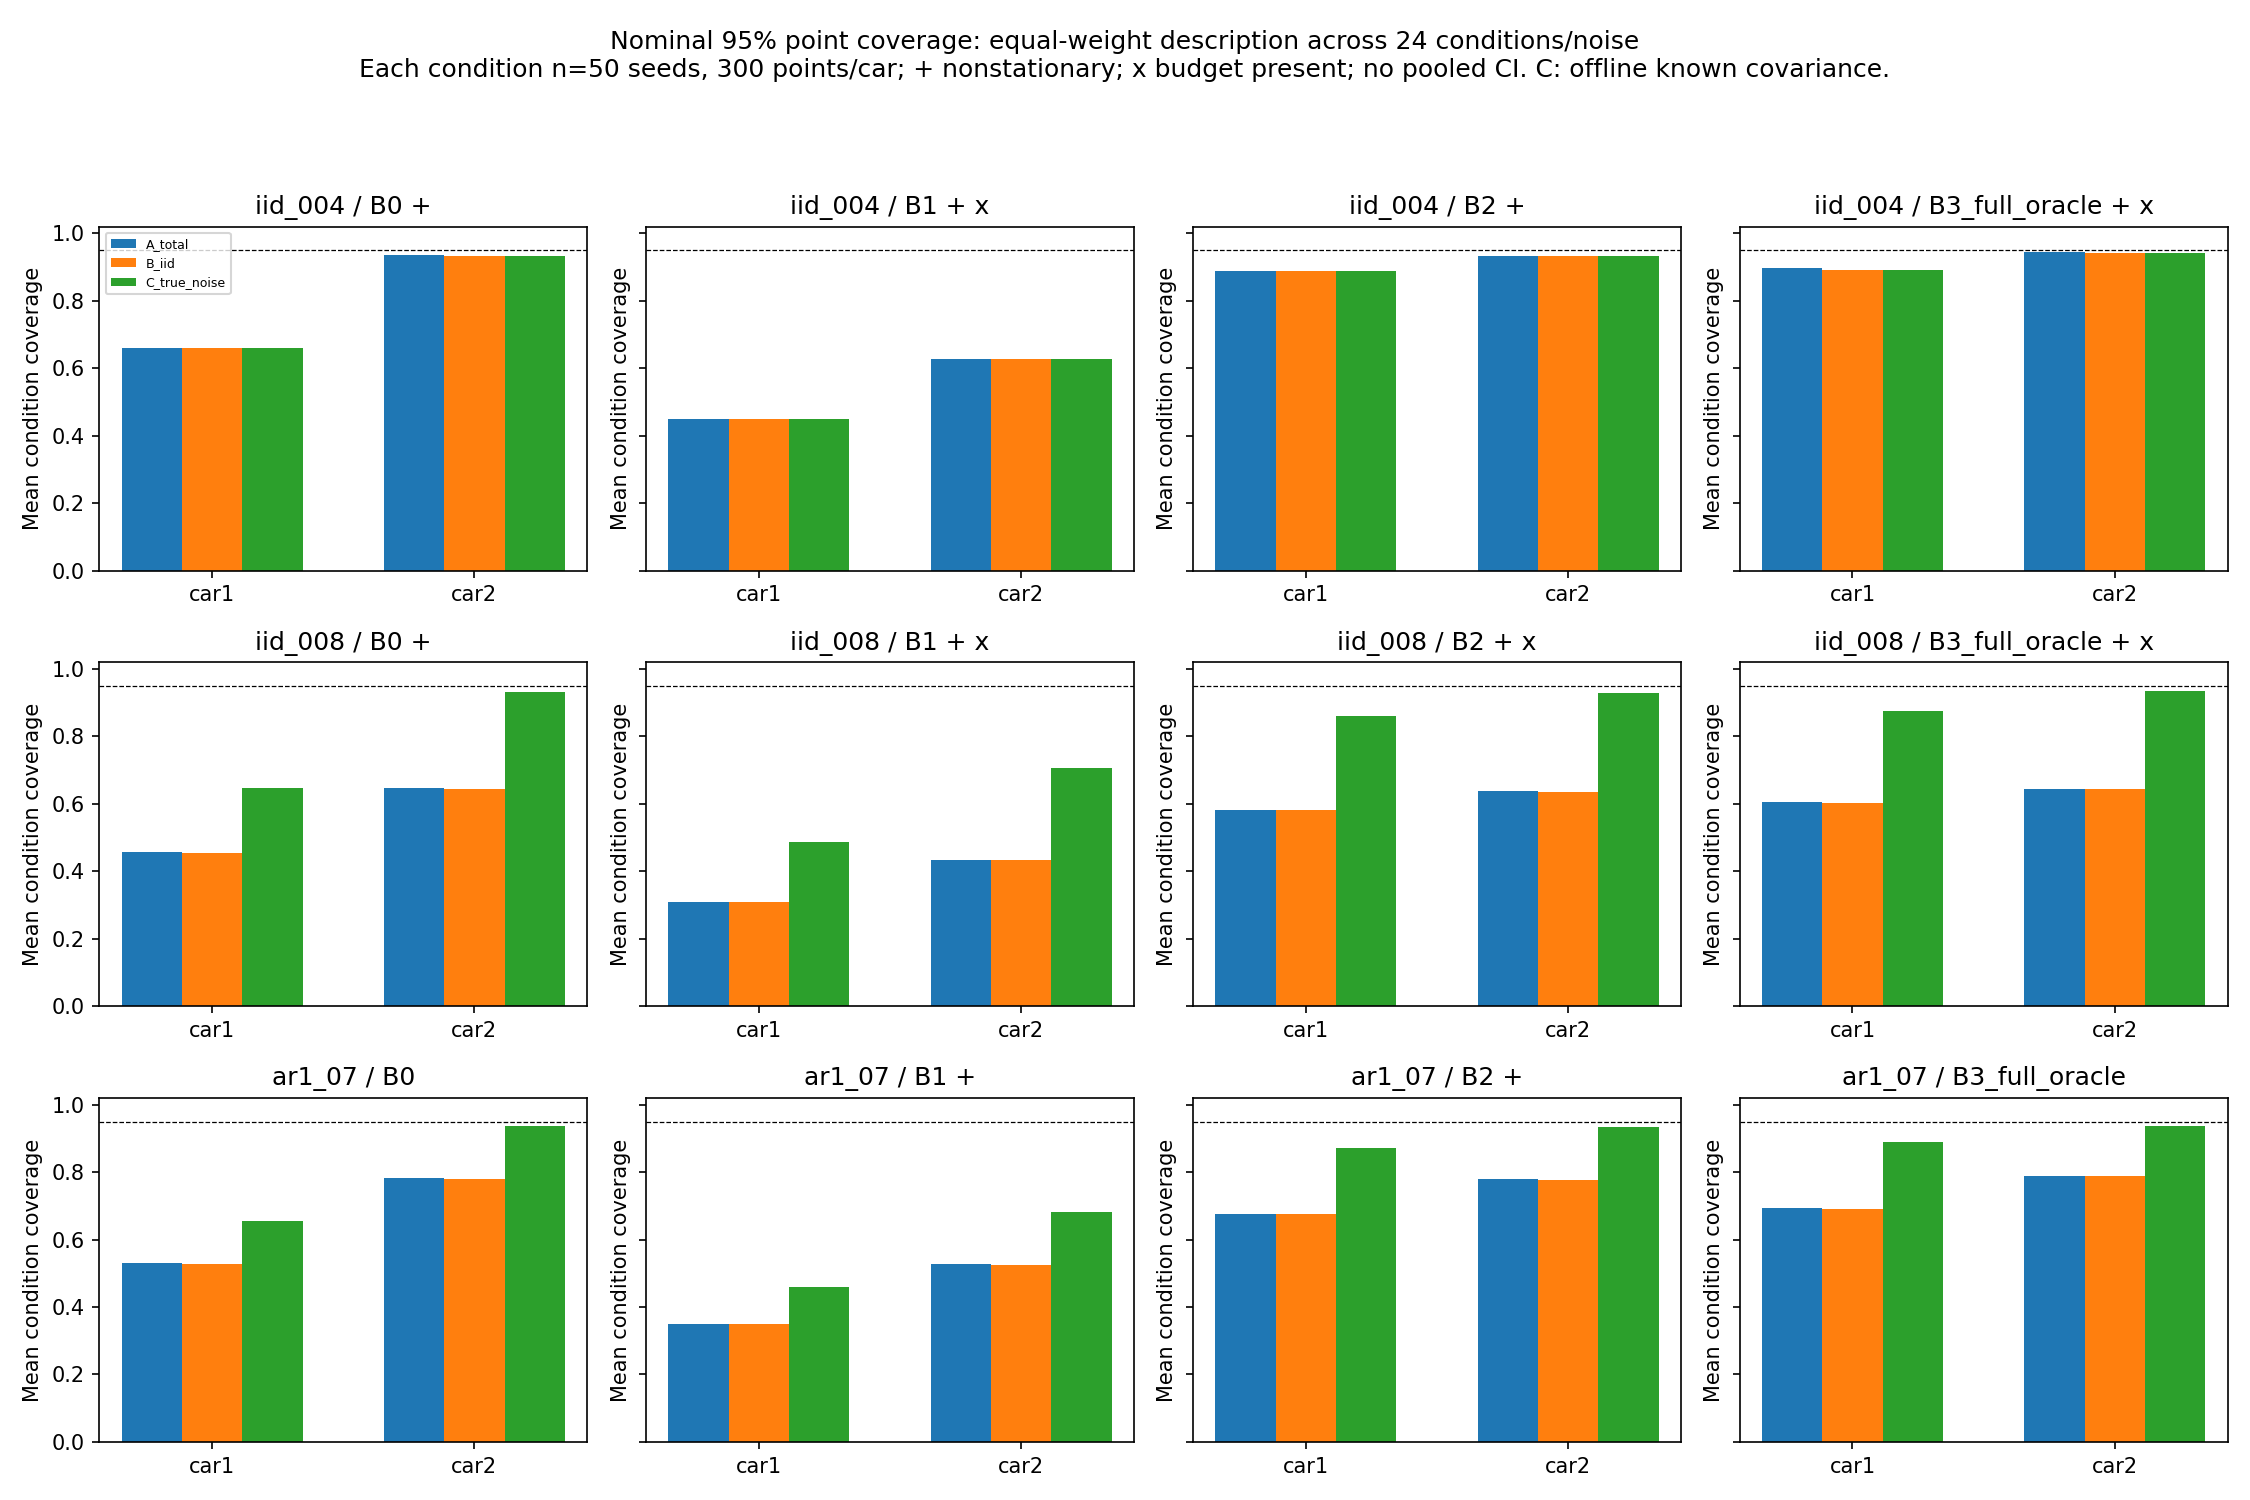
\includegraphics[keepaspectratio,alt={图4-1
三种噪声下四方法的两车覆盖与传播矩阵比较}]{figures/noise_explanations.png}}
\caption{图4-1 三种噪声下四方法的两车覆盖与传播矩阵比较}
\end{figure}

图4-1原样复用 R108 的完整噪声解释图：每种噪声包含24条件，各条件50个独立
seed，每车点平均分母300。柱高是条件覆盖率的等权描述均值，无跨条件堆叠置信区间；三色分别为总曲率、独立噪声传播与真实协方差传播，虚线为名义95\%。标题中的``+''与``x''标记该组含未驻点和预算耗尽，均保留在统计中。真实协方差仅作离线理想诊断，估计位置没有随矩阵变化；各方法、两车和不利结果均保留。

已知真实协方差解释了一部分欠覆盖，但仍留下明确反例。n32（weak / static /
peer / zero，AR）的车1
C覆盖为221/300，即73.67\%，seed簇95\%区间为61.33--84.67\%；同车六时刻全覆盖为34/50，车2为43/50。该条件车1平均
MSE约0.06190 m²，经验均值误差平方约0.03791 m²，C预测迹约0.05714
m²。即使平均尺度与 MSE 接近，中心、方向及分布形状仍可能不符；trace
的接近不能替代椭圆事件的逐点核验。{[}R108 §4，噪声 COVERAGE/MOMENTS
表，n32 / B2 / C\_true\_noise{]}

残差也不能单独承担可信性判断。相同弱静止 peer 零注入场景中，B2 在 AR
噪声下的平均总白化残差 RMS 从独立0.04 m时约0.78181降为0.70694，车1平均
RMSE反而从0.15545 m升至0.20425
m。后续覆盖分析另列``数据残差''，去掉先验行后数值有所不同，不能混用两种定义。这里仅展示相关噪声可被状态部分拟合的现象，没有据残差搜索事后最优告警阈值。{[}R107N
§3；R108 §5{]}

\subsection{4.5
先验机制对照：固定错误中心与非线性缺口并存}\label{ux5148ux9a8cux673aux5236ux5bf9ux7167ux56faux5b9aux9519ux8befux4e2dux5fc3ux4e0eux975eux7ebfux6027ux7f3aux53e3ux5e76ux5b58}

\subsubsection{4.5.1
在相同观测和初值上改变什么}\label{ux5728ux76f8ux540cux89c2ux6d4bux548cux521dux503cux4e0aux6539ux53d8ux4ec0ux4e48}

先验机制批次使用三种几何、peer零/0.3 m注入、0.5/0.05
m两种先验标准差，以及 fixed\_correct、fixed\_survey、random\_correct
三种中心机制，共36条件、每条件100个新 seed。fixed\_correct
把先验中心固定在真值；fixed\_survey 使用原有错误 survey；random\_correct
在真实首时刻位置上增加与先验标准差匹配的独立 Gaussian
随机量。所有组初值固定为原 survey
加同一带噪全局位移积分，不因中心变好而同步得到更好的初始化。{[}R109
\texttt{PROTOCOL.md}{]}

两种 correct
均利用仿真真值，属于理想诊断机制。随机正确中心与固定正确中心不是同一种频率模型：前者每次重复重新采样先验观测，后者的中心在重复中不动。改变
random\_correct
的标准差同时改变先验观测精度和权重，不能称为固定观测下的纯权重扫描。truth\_linearized
则在真值处构造仿射残差并直接求解，逐输入配对非线性估计；其用途是检验传播公式和隔离一阶近似，不能部署在未知真值上。{[}R109
\texttt{PROTOCOL.md}``三种量的推导''{]}

\subsubsection{4.5.2
错误强先验足以产生严重欠覆盖}\label{ux9519ux8befux5f3aux5148ux9a8cux8db3ux4ee5ux4ea7ux751fux4e25ux91cdux6b20ux8986ux76d6}

表4-5保留 weak/static/peer \(+0.3\) m、B2 的全部六种先验组合。MSE为车1逐
seed 均值，单位 m²；覆盖为总曲率椭圆的95\%点平均，两车分别列出。每格独立
\(n=100\)，每车覆盖分母600，未驻点有限解保留；线性和非线性结果共享样本。本表没有只挑中心正确的有利组。{[}R109
\texttt{results/SUMMARY.csv}，p18--p23/B2；\texttt{results/COVERAGE.csv}，curvature
/ all / point\_average / 0.95{]}

{\def\LTcaptype{none} % do not increment counter
\begin{longtable}[]{@{}
  >{\raggedright\arraybackslash}p{(\linewidth - 8\tabcolsep) * \real{0.1579}}
  >{\raggedleft\arraybackslash}p{(\linewidth - 8\tabcolsep) * \real{0.2105}}
  >{\raggedleft\arraybackslash}p{(\linewidth - 8\tabcolsep) * \real{0.2105}}
  >{\raggedleft\arraybackslash}p{(\linewidth - 8\tabcolsep) * \real{0.2105}}
  >{\raggedleft\arraybackslash}p{(\linewidth - 8\tabcolsep) * \real{0.2105}}@{}}
\toprule\noalign{}
\begin{minipage}[b]{\linewidth}\raggedright
先验标准差 / 机制
\end{minipage} & \begin{minipage}[b]{\linewidth}\raggedleft
车1线性 MSE
\end{minipage} & \begin{minipage}[b]{\linewidth}\raggedleft
车1非线性 MSE
\end{minipage} & \begin{minipage}[b]{\linewidth}\raggedleft
线性覆盖：车1 / 车2
\end{minipage} & \begin{minipage}[b]{\linewidth}\raggedleft
非线性覆盖：车1 / 车2
\end{minipage} \\
\midrule\noalign{}
\endhead
\bottomrule\noalign{}
\endlastfoot
0.5 / 固定正确 & 0.001224 & 0.017877 & 99.00\% / 99.17\% & 90.67\% /
89.50\% \\
0.5 / 固定survey & 0.064239 & 0.020135 & 99.00\% / 98.67\% & 87.33\% /
87.83\% \\
0.5 / 随机正确 & 0.244438 & 0.022563 & 96.33\% / 93.50\% & 86.83\% /
89.33\% \\
0.05 / 固定正确 & 0.001217 & 0.001265 & 99.17\% / 99.00\% & 98.83\% /
98.83\% \\
0.05 / 固定survey & 0.064287 & 0.048938 & 0.67\% / 6.67\% & 1.83\% /
10.00\% \\
0.05 / 随机正确 & 0.003236 & 0.003345 & 96.00\% / 96.17\% & 95.50\% /
96.33\% \\
\end{longtable}
}

固定 survey 强先验的车1非线性 MSE为0.048938 m²，其中跨 seed
均值误差平方的六时刻均值为0.047726
m²，约占97.5\%；主要问题是均值偏移。只把中心改为正确位置，保持权重、观测和初值不变，车1
MSE降至0.001265 m²。survey−correct 的配对 MSE差为0.047673
m²，95\%逐项区间为{[}0.045531, 0.049913{]} m²。{[}R109
§2，MOMENTS、PAIRED\_COMPARISONS 表{]}

同一强 survey
组的100个非线性结果全部数值接受，却只有1.83\%/10.00\%的点覆盖；其线性结果也严重欠覆盖。因此固定错误中心本身足以构造问题，并不需要求解器失败才能解释。反过来，不能将该比例推广到所有欠覆盖组：0.5
m温和 survey
的线性曲率覆盖接近99\%，非线性约87\%，说明还有其他作用。{[}R109
§§2--3{]}

\subsubsection{4.5.3
中心正确仍不保证局部曲率覆盖}\label{ux4e2dux5fc3ux6b63ux786eux4ecdux4e0dux4fddux8bc1ux5c40ux90e8ux66f2ux7387ux8986ux76d6}

weak、fixed\_correct、0.5
m的车1非线性覆盖为90.67\%，seed簇95\%区间{[}86.00\%,94.67\%{]}，车2为89.50\%；线性分别99.00\%和99.17\%。非线性−线性的车1覆盖差为−8.33个百分点，逐项区间{[}−13.00,−4.33{]}个百分点。即使只看98个数值接受
seed，覆盖仍为90.48\%和89.46\%。这排除了``全部欠覆盖只来自未驻点''的解释，但没有证明这些解都是全局最优。{[}R109
§3{]}

这里线性 fixed\_correct
的约99\%不能直接当作``名义95\%被准确复现''：固定中心的实际波动不含先验重采样，而候选总曲率逆包含先验信息的随机解释，因而可保守。正确指定的
random\_correct
线性组才具有与曲率传播匹配的随机先验机制，其理论点态覆盖为95\%；固定正确中心使用相应数据噪声传播、且二维块可用时，也有相应线性理论解释。报告同时保存解析覆盖，不用100个
seed 的经验值替代理论概率。{[}R109
§1，\texttt{LINEAR\_ANALYTIC\_COVERAGE.csv}{]}

\begin{figure}
\centering
\pandocbounded{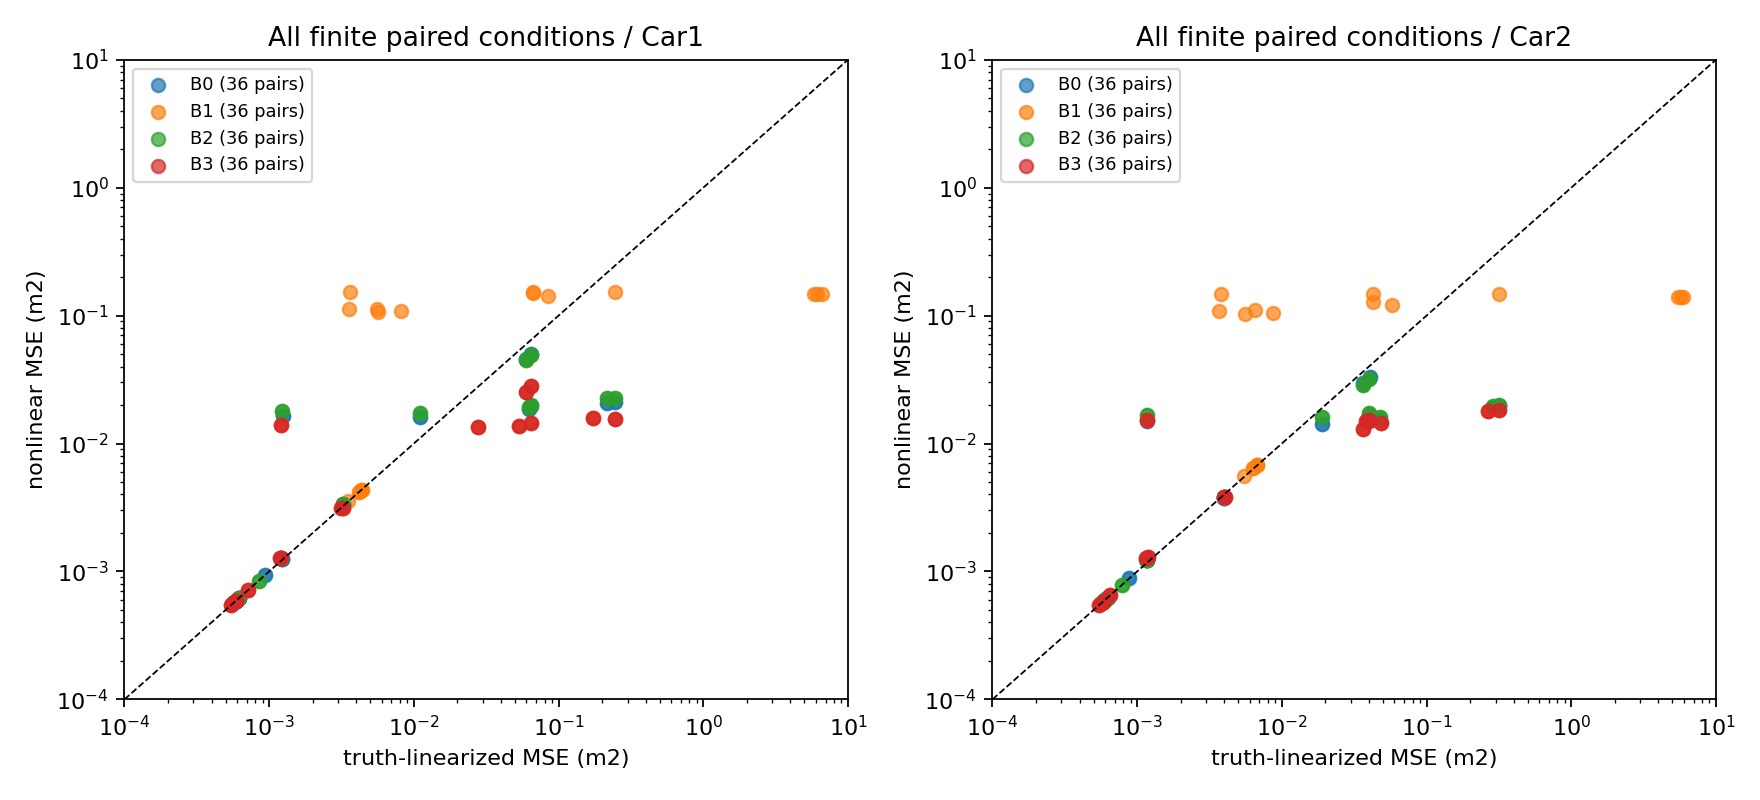
\includegraphics[keepaspectratio,alt={图4-2
全部条件的真值处线性诊断与非线性 MSE
对照}]{figures/prior_linear_nonlinear_full_range.png}}
\caption{图4-2 全部条件的真值处线性诊断与非线性 MSE 对照}
\end{figure}

图4-2复用固定提交 R109 原图：横轴为真值处线性化 MSE，纵轴为非线性
MSE，左右分别为车1、车2；每种方法36个条件点，每点由100个独立 seed
的六时刻 MSE取均值。图为双对数坐标，虚线为相等线，保留超过1
m²的极端线性结果及所有有限非线性结果。条件、方法和车辆之间相关，不将图点数当独立样本，也不据散点宣称线性诊断可部署或总体更好。两车完整曲率覆盖热图见
\texttt{FIGURE\_TABLE\_INDEX.md} 的F03a/F03b。

在 weak、random\_correct、0.5 m中，车1线性 MSE约0.24444
m²，非线性约0.02256
m²，后者误差更小却覆盖更低。真值处共线测距对横向扰动的一阶导数为零，但有限横向扰动仍改变真实距离；一阶对照并不保留全部高阶信息。现有差异可能同时包含高阶曲率、随数据改变的
Jacobian、局部分支、固定 survey
初值及数值残留。本批没有逐项干预隔离这些机制，不能将散点差异全部归因于某一个原因。{[}R109
§5{]}

\subsection{4.6
失败、不可用与完整矩阵的保存原则}\label{ux5931ux8d25ux4e0dux53efux7528ux4e0eux5b8cux6574ux77e9ux9635ux7684ux4fddux5b58ux539fux5219}

原正式确认的7200次方法运行包含25个未驻点；故障28800次包含367个未驻点和14个P1预算耗尽；噪声14400次包含333个未驻点和20个P1预算耗尽；先验机制14400次非线性运行包含65个未驻点。各批最终估计均有限且无缺失，主误差与覆盖统计保留这些终点。未驻点不是``已接受''，预算耗尽也不是``无估计''；把它们整体删除会改变所评估的算法行为。{[}R0、R107F/N、R109
的完成表及 NONACCEPTED/FAILURES{]}

先验机制的总状态信息均满秩，但两个模型类型、两种矩阵视图共691200个二维位置块中，6400个固定中心
weak
真值线性对照的首时刻噪声传播块奇异。这是某些方向在该传播机制下确定、二维椭圆不可用，不是总解必然不唯一。协议以
SINGULAR\_MARGINAL
记录，不使用伪逆填出有限椭圆；其余684800块可用。95\%与99\%共享可用性，不能因为改变名义级别就消除奇异。{[}R109
\texttt{REPORT.md}``实际完成与核验''；\texttt{PROTOCOL.md}{]}

正文只保留能够解释研究问题的表和图，完整矩阵由证据附件索引：原批的36条件、故障和噪声各72条件、先验机制36条件，以及四方法、两车、矩阵视图、95\%/99\%、逐点/点平均/轨迹事件和数值子集。极值案例按原协议规则选择，未因对
B2
不利而删除。未观察到某一类异常不等于它的总体概率为零，数百或数千方法调用也不能绕过共享
seed 获得罕见风险证据。

\section{5
适用边界与后续技术路线}\label{ux9002ux7528ux8fb9ux754cux4e0eux540eux7eedux6280ux672fux8defux7ebf}

\subsection{5.1
当前已经建立的证据链}\label{ux5f53ux524dux5df2ux7ecfux5efaux7acbux7684ux8bc1ux636eux94fe}

本阶段建立的是限定条件下的方法和不确定性诊断链。实测说明协同影响具有逐车差异；单常值仿真说明偏差可以在指定链路上进入状态并减轻漏建模误差；信息分析说明整体局部秩、偏差有效信息和有限噪声精度必须分开；覆盖分析说明可逆曲率矩阵、数值接受及较小误差都不能单独推出可信区间。三类来源互相补充，但不共享同样的真值质量或随机模型。{[}第2--4章及
CLAIM\_EVIDENCE{]}

已有结果支持条件性的技术判断：候选正确且故障满足单常值假设时，B2相对被污染
B1
有明确改善；候选错误、额外故障或时间变化时，该收益可能减弱甚至反向。固定错误强先验能够造成均值偏移和严重欠覆盖；真实噪声协方差的离线传播能解释部分随机尺度失配，却不能消除模型均值漏项；正确先验中心下的弱几何非线性缺口仍存在。这些判断均附适用条件，不扩写为任意
NLOS 的解决方案。{[}R107F；R108；R109{]}

现有仿真中正确中心、真值处线性化、已知真实噪声协方差和 B3
都有真值信息边界。它们帮助定位``哪个假设可能失效''，并不自动提供实车可使用的信息。室内静态/有限动态材料与六时刻仿真均不是月面环境验证；研究题目的月球探索目标在本阶段体现为后续系统约束，而非已经完成的环境适应性结论。

\subsection{5.2
从诊断模型到可部署协同定位的缺口}\label{ux4eceux8bcaux65adux6a21ux578bux5230ux53efux90e8ux7f72ux534fux540cux5b9aux4f4dux7684ux7f3aux53e3}

首先需要解决故障候选的依据。当前 B2
的候选由实验设计给定；一旦未知链路、多链路和时变偏差并存，候选选择错误本身就会进入误差预算。后续可以研究有限故障假设集合、可检测性与候选拒判，但应先冻结候选集合和未覆盖故障类别，再评价方法；不能在本批结果上选择效果最好的候选后回报收益。现有结果没有估计未知候选被正确选择的概率。{[}R107F
§§3--4；R108 §1{]}

其次需要建立先验的外部依据。固定 survey
的误差跨重复不重新采样，随机先验则要求明确独立测量过程；两者在实际系统中可能同时存在。需要从布设、外部定位或历史状态来源解释中心误差、随机成分及其与当前观测的相关性。若先验由同一传感器历史数据产生，还应避免重复使用信息。理想
correct
对照只能作为上限或机制参照，不能充当实际先验已被校准的证据。{[}R109
§§1--4{]}

第三是运动与相关噪声。当前运动数据直接约束全局二维位移，省略未知航向、轮速尺度误差、IMU偏置、时间对齐及预积分相关性。在这样的简化模型上得到的可辨识性和覆盖结论，需要在扩展状态与实际因子定义下重新核验。AR(1)只是六时刻的受控相关噪声机制，不能代表已经完成现场噪声谱或长时间相关估计。噪声模型应来自独立数据，验证数据不应同时用于调节传播阈值和宣称达到覆盖。{[}R0
局限；R107N 协议及结论{]}

\subsection{5.3
A端非线性诊断的预留位置}\label{aux7aefux975eux7ebfux6027ux8bcaux65adux7684ux9884ux7559ux4f4dux7f6e}

\textbf{预留接口
A-NL：在本节之后插入新的、独立固定提交的非线性机制诊断结果。当前状态为计划，不纳入本报告已完成运行数。}
需要回答的具体问题是：在先验中心和生成机制已控制后，weak/near
的位置分支、高阶曲率和终点 Jacobian
变化分别解释多少剩余欠覆盖，而不是再次证明已经知道的``弱几何误差较大''。{[}由
R109 §5 提出的待解问题{]}

建议交付至少保留同输入的目标值、物理梯度、初始化规则、最终状态分支与误差、局部矩阵以及失败标签。若采用多初值，只能使用预先规定、与未知真值无关的选解规则；多初值调用数与独立
seed 数分别报告。若比较精确
Hessian、高阶传播或不同参数化，应同时检查矩阵可用性和模型假设，不能只保留更接近名义覆盖的方案。接受子集与全计划结果并列，防止把数值筛选误写成算法改进。

插入结果时必须给出新协议冻结点、与本报告的共享输入关系、完整条件索引和对原结论的影响。若只做保存状态上的诊断，应明确新增优化调用为零；若确需新优化或新观测，则独立登记，不能计入当前完成数。当前
C端不等待该窗口，也不代写其尚未获得的结果。

\subsection{5.4
B端先验传播分析的预留位置}\label{bux7aefux5148ux9a8cux4f20ux64adux5206ux6790ux7684ux9884ux7559ux4f4dux7f6e}

\textbf{预留接口
B-PRIOR：在本节之后插入实际先验来源与传播分析。当前仅保留问题、变量定义和验收要求，不提前写入数值结论。}
重点应从``选哪个先验标准差使覆盖较好''转为``先验中心怎样生成，哪些成分固定，哪些成分随机，哪些与当前测量相关''。{[}由
R108 §4、R109 §§1--4提出的待解问题{]}

后续需要区分条件于固定中心的随机波动、先验中心误差引起的偏移，以及跨中心重复的总波动；若允许相关性，必须显式给出交叉协方差及其来源。只增大区间尺寸并不能说明概率语义正确。对比应保留估计中心不变与重新加权求解之间的区别，避免将离线传播矩阵的改善写成定位误差改善。

交付验收可包括解析小模型、固定与随机中心的一致性检查、误差均值与中心协方差分解、可用区间/全计划分母、以及对实际数据先验来源的可追溯说明。这些是后续技术要求，不代表本窗口已实现新的先验传播算法，也不把当前真实
\(\Omega\) 的理想结果转换为在线能力。

\subsection{5.5
完好性目标的表述与阶段定位}\label{ux5b8cux597dux6027ux76eeux6807ux7684ux8868ux8ff0ux4e0eux9636ux6bb5ux5b9aux4f4d}

本文统一将 integrity
译为``完好性''。当前经验95\%/99\%覆盖评估的是指定模型、指定样本和局部候选区间的一致性；尚未定义并验证满足任务风险要求的保护级
PL、HCPL 或危险误导信息 HMI
保证。点态失覆盖率、轨迹全覆盖比例和安全风险也不是同一事件。未来若开展完好性设计，应先明确告警限、风险事件、时间范围、故障假设与不可用输出规则，再讨论如何在独立证据上验证。

师兄方案的原始公式、假设或风险分配若不能从原文件核实，相关推导必须保持缺失状态；不能根据聊天摘要补造公式编号、HCPL表达式或已经满足的风险阈值。本阶段更稳妥的交付是：明确哪些模型条件下已有条件性定位收益，哪些区间已经出现可复核失效，以及后续需要哪些独立输入才能推进完好性量化。技术正文与完整证据附件分开，便于后续窗口逐项替换待确认内容，而不改写已冻结的实验事实。
\end{document}
